\documentclass[a4paper,american,12pt]{article}
\usepackage{graphicx}
\graphicspath{{images/}}

%************************** Language and font encodings **************************
\usepackage[utf8]{inputenc}

%************************** Sets page size and margins **************************
\usepackage[top=2cm,bottom=2cm,left=2cm,right=2cm,marginparwidth=1.75cm]{geometry}
\setlength{\parskip}{1em}

%************************** Useful packages **************************
\usepackage{amsmath}
\usepackage{graphicx}
\usepackage{subcaption}
\usepackage{float}
\usepackage[colorlinks=true, allcolors=black]{hyperref}
\usepackage{csquotes}
\usepackage{graphicx}
\usepackage{setspace}
\usepackage[noconfigs,british]{babel} 

%************************** List of abbreviations **************************
\usepackage{acronym}

%************************** Specify bibliography package **************************
\usepackage{csquotes}% Recommended
\usepackage[style=apa]{biblatex}
\DeclareLanguageMapping{american}{american-apa}
\addbibresource{references.bib}

%************************** Section Title Margins **************************
\usepackage{titlesec}
\titlespacing*{\section}
{0pt}{3.0ex plus 1ex minus .2ex}{0.7ex}
\titlespacing*{\subsection}
{0pt}{1.4ex}{0pt}
\title{Review of Assigned Readings}
\author{Your Name Goes Here}
    
    
%************************** DOCUMENT_STARTS_HERE **************************
\begin{document}

%************************** Title Page **************************   
\begin{titlepage}
	\begin{figure}
	\centering
	
\includegraphics[scale=0.32]{logohsg}
	\end{figure}
\centering
{\scshape\large School of Management, Economics, Law, Social Sciences and International Affairs \par}
\vspace{2.0cm}
{\huge\bfseries The effect of Twitter activity on Bitcoin price fluctuation  \par}
\vspace{2.0cm}
{\scshape\Large Software Engineering for Economists \\(7,610,1.00) \par}
\vspace{2.0cm}
{\itshape\large Alen Stepic - 11-475-258 \\Dimitrios Koumnakes - 10-613-370 \\Joël Sonderegger - 11-495-488 \\Severin Kranz - 13-606-355 \\Chi Xu - 16-300-915 \par}
	\begin{spacing}{1}
	\vspace{1.2cm}
	{Fall Term 2017 \par}
	\vspace{1.2cm}
	Supervisor:\\
	{Prof. Dr. Philipp Zahn\\ FGN HSG\\ Varnbüelstrasse 19\\ 9000 St. Gallen \par}
	\end{spacing}
\vfill
{\large \today\par}
\end{titlepage}
    
\clearpage
    
%************************** Abstract ************************** 
\begin{abstract}
\pagenumbering{Roman}
This paper, examines the dynamics between the amount of twitter activity regarding bitcoin and the actual price fluctuation of bitcoin. For the analysis two sets of data have been collected. One reflecting twitter activity and the other one showing the bitcoin prices for the same period. Based on that an econometric model is used for the statistical analysis and the interpretation of the results.\\
The evaluation of the model showed that changes in twitter activity on bitcoin have a minimal and insignificant effect on the future price development of bitcoin. Accordingly, aggregate twitter fees are not a good source to predict changes in bitcoin prices. This result must be understood with caution, because it only applies for the specific time interval of our observations, which is about 8 days and not for the past or future trend of cryptocurrencies. \\
This work was created in the context of a programming course for economists at the university of St. Gallen. To not exceed the framework of this study we require extensive knowledge in econometrics and take concepts as known. The underlying goal was to get familiar with software engineering tools and project management. Therefore, the academic content of this work is neither completed nor concluding.\\
\end{abstract}

\clearpage

%************************** Contenttable Page ************************** 
\tableofcontents

\clearpage

%************************** List of Figures ************************** 	
\listoffigures\bigskip\bigskip
\listoftables
 	   
\section*{List of Abbreviation} 
\begin{acronym}[ASECRETTT]
\acro{VAR}{Vector Autoregression}
\acro{EMH}{Efficient Market Hypothesis}
\acro{etc}{et cetera}
\end{acronym}

\clearpage

%************************** Chapters 1 - Introduction **************************
\begin{spacing}{1.2}
\cleardoublepage\pagenumbering{arabic}
\section{Introduction}
\label{sec:intro}
\textcite[p.~388]{malkiel1970efficient} introduced the Efficient Market Hypothesis (EMH), where they claim that under certain market conditions actual prices include all information. This hypothesis is broadly accepted in the financial world. The digitalisation leads to an increased network effect, where information can be shared over the globe. Based on \citeauthor{mao2015quantifying} (\citeyear[][p.~3]{mao2015quantifying}, as cited in \cite[][pp.~175--195]{shiller2015irrational}; \cite[][pp.~279]{kahneman2013prospect}) the EMH fails to address the behavioural and emotional role of investors. The large fluctuation of the bitcoin prices in the last year (mostly increasing) and the fact that Twitter has become a very popular social network, where people interact, led to different research in the field of sentimental analysis with the focus on bitcoin and twitter. \textcite[p.~18]{mao2015quantifying}, claim that sentiment analysis using twitter tweets which contain the buzzword bullishness can indeed be used as a sentiment indicator for stock prices. As modern economy becomes more digitized, crypotocurrencies as a financial asset draws more attention, our paper seeks to shed some light on whether the tweets can be used to predict bitcoin prices.

\subsection{Research Question and Goal of the Paper}
\label{sec:ResearchQandGoal}

As existing research focus mostly on the sentimental analyses of tweet content, this paper aims to examine existence of a correlation between the price development of bitcoin and the frequency of bitcoin topics on twitter. The goal should be reached by answering the following research question: \\
In what extend does the amount of twitter tweets about bitcoin has an effect on the price movement of bitcoin?

\subsection{Methodology}
\label{sec:Methodology}
To answer the above mentioned research question a scientific approach has been applied. The paper consists out of three parts. The first part contains an introduction into the topic by pointing out the relevance of the topic, the research question, methodology and the scope. This is conducted in chapter \ref{sec:intro}. The second part is characterized as the theory part. The theory aims to provide the reader with the necessary background information by introducing relevant bitcoin and twitter information in context of the paper. The conducted research is based on forward research and using relevant sources. Furthermore, it contains a short introduction into the Vector Autoregression (VAR) approach and its constrains in context with the paper. This is conducted in chapters \ref{sec:Background} and \ref{sec:EconometricModellingandResults}. The third part contains the discussion of the results and a conclusion. The conclusion is based on the theory and our mathematical computation. The computation is based on a data set, which was gathered by coded python scripts for the time period December 20th - 27th. Since the results are based on the observation of a short period, they have to be interpreted carefully. The data set consists of two data sources with the following characteristics: (1) twitter tweets which contain the buzzword "bitcoin" and (2) those containing historical bitcoin prices. The two sources has been aggregated with another python script. The output of aggregation was further processed with Stata to conduct the VAR on a daily basis. The third part of the paper is discussed in the chapters \ref{sec:EconometricModellingandResults} and \ref{sec:Conclustion}.

\subsection{Scope}
\label{sec:Scope}
The paper's focus lies on the scientific discussion of empirical test results. The research question has consciously been narrowed down, as the focus of the course Software Engineering for Economists is the application of different tools, the documentation and reproducibility of the results, rather than writing a high-quality scientific paper. As already mentioned above, the results have to be interpreted carefully because of the limited observation period of seven days. The approach and technical issues (like code scripts etc.) are not addressed, for purposes we shall address in the separate documentation paper.

\clearpage

%************************** Chapters 2 - Background and Data Collection **************************
\section{Background and Data Collection}
\label{sec:Background}
\subsection{Bitcoin}
In the aftermath of the global financial crisis, Satoshi Nakamoto (2008, p. 1) claimed, that a purely peer-to-peer version of electronic cash could bypass financial institutions as third parties for commercial transactions. Starting from this whitepaper, Bitcoin – the first electronic payment system that relies on the cryptographic concatenation of ongoing transactions \footnote{blockchain} has been developed (Nakamoto, 2008, p. 1).\\

Today, Bitcoin is the most popular of thousands of cryptocurrencies worldwide and increased in value over 1700 percent within the last year according to Coinmarketcap (https://coinmarketcap.com/). Even if the daily transaction volume increased rapidly over time (https://coinmarketcap.com/), this does not necessarily mean that Bitcoin is used for payment purposes. Even more, several authors argue that the Bitcoin price and transaction volumes are mainly pushed by speculative investments rather than actual usage as a currency (Corbet, Lucey \& Yarovya, 2017; Forbes, 2017; Yermack, 2013). Kristoufek (2015) points out that there are other influencing factors such as usage in trade, money supply and price level, that influence the Bitcoin price in the long term. However, evidence shows that the level of Bitcoin prices are clearly driven by investors’ interest in the digital currency. Kristoufek (2015) further explains the correlation is most evident in the long run.  During explosive increases or rapid declines of the price higher investors’ interest further boosts the movement in the direction (Kristoufek, 2015). These findings are in line with other researchers (see Garcia, Tessone, Mayrodiev \& Perony, 2014; Kondor, Posfai, Csabai, \&Vattay, 2014).\\

In previous research Madan,Saluja, and Zhao (2015)applied \textit{machine learning} algorithms to predict Bitcoin prices. By using the \textit{Bayesian regression}, Shah, Devavrat and Zhang (2015) achieved a return on investment of 89 percent over an investment period of 50 days. However, research in this area is still limited and most of them do not take into consideration the individuals' sentiments (Colianni, Rosales \& Signorotti, 2015, p. 1).\\

One core assumption of behavioural finance is that investors’ interests influence their behaviour and therefore stock prices(Mao et al., 2015, p. 3). A widely used approach to measure investors’ interests is the sentiment analysis of Twitter data, which will be covered in the following section.\\
		
\subsection{Twitter}
With the current growth of social networks, the number of global social media users reached 2.46 billion and is expected to increase to 3.02 billion by 2021 according to Statista (2018). Gabriel and Röhrs (2017) define social networks as a loose connection of people in an online or internet community, respectively in a computer-based communication network (p. 12). This paper exploits the possibility to analyse shared “thoughts, views and opinions” (Stenqvist and Lönnö, 2017, p. 6) provided by such communities or communication networks.\\

Twitter was founded in 2006 and gained rapidly worldwide popularity (Twitter 2018). and reached 330 million active users in the third quarter of 2017 (Twitter 2017, Statista 2018). As a micro-blogging platform, Twitter suits the purpose of analysing investors’ interests due to its special characteristics. In comparison to other social networks, twitter limits its posts (tweets) to relatively short messages of 140 characters. Tweets can contain observations, thoughts, links to interesting content, websites, uploaded pictures or videos. Special conventions such as hashtags “\#” or mentions “@” are used to reference searchable content or user profiles.(Schmidt, 2017)\\

In this way, Twitter users create millions of posts that contain interests, opinions and informations in both a private and professional context.  Due to the semi-structured form, the message length restriction and classifying nature, Stenqvist and Lönnö (2017, p. 6) argue, that “Twitter has become a gold mine for opinionated data”, which is further supported in the wide adoption of researchers to analyse sentiments.\\

In relation to Bitcoin,researchers already showed that analysing investors sentiments can lead to reasonable correlations between Twitter sentiments and prices of cryptocurrencies (Stenqvist and Lönnö, 2017, p. 7), by either using a \textit{polarity classification} – classifying the language in tweets as either positive or negative (see Colianni et al., 2015) – or a \textit{lexicon based approach} – attributes predefined words to specific sentiment classifications (see Stenqvist and Lönnö, 2017). Hence, this paper choses a different focus area by limiting its scope to the number of daily tweets that contain the term “Bitcoin” without analysing investors interests any further. Based on analysis of the influence of twitter bullishness on the stock market by Mao et al. (2015), this paper further elaborates on the concept by applying the approach to Bitcoin prices.\\


		
\subsection{Data Collection}
For our data, we collected 2 separated time series datasets. One showing the twitter activity regarding bitcoin and the second one showing the bitcoin price development. Both datasets, were collected hourly for the period from the 19.12.2017 starting at 20:00:00 UTC and ending on the 28.12.2017 at 10:00:00 UTC. We chose the hourly basis to be able to do a statistical analysis with a certain amount of observations in the restricted processing time for this homework. For the twitter data we aggregated every hour the total number of tweets mentioning bitcoin. For the bitcoin prices we selected prices at the last second of every hour.\\
The following figure displays the twitter activity regarding bitcoin for the observed time period. The first plot shows the hourly change of the aggregate number of tweets containing bitcoin. In the second and third plots we did a first difference and a logarithmic first difference transformation of our main variable, in case it is needed in the later analysis. The graphs show overall a cyclical movement arount 1200 tweets and a single outburst on the 22.12.2017 for the time interval between 15:00:01 and 21:00:00 with highest value being 4622 tweets in one hour.\\

\begin{figure}[H]
	\begin{subfigure}{.3\textwidth}
	\centering
	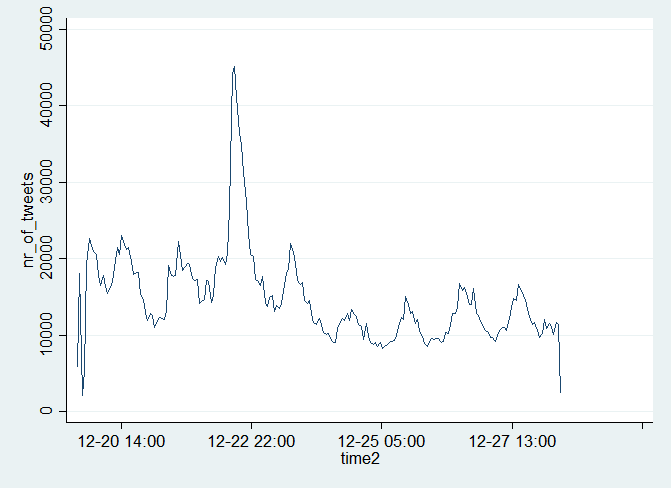
\includegraphics[width=1.12\textwidth]{stata_export_graphs/graph_plot_nr_tweets.png}
	\caption{Number of Tweets regarding bitcoin}
	\end{subfigure}\hfill
	\begin{subfigure}{.3\textwidth}
	\centering
	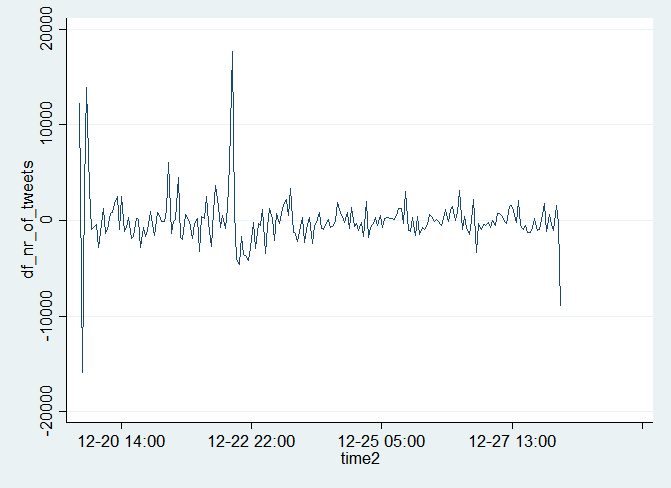
\includegraphics[width=1.12\textwidth]{stata_export_graphs/graph_plot_df_nr_tweets.png}
	\caption{First difference of number of Tweets}
	\end{subfigure}\hfill
	\begin{subfigure}{.3\textwidth}
	\centering
	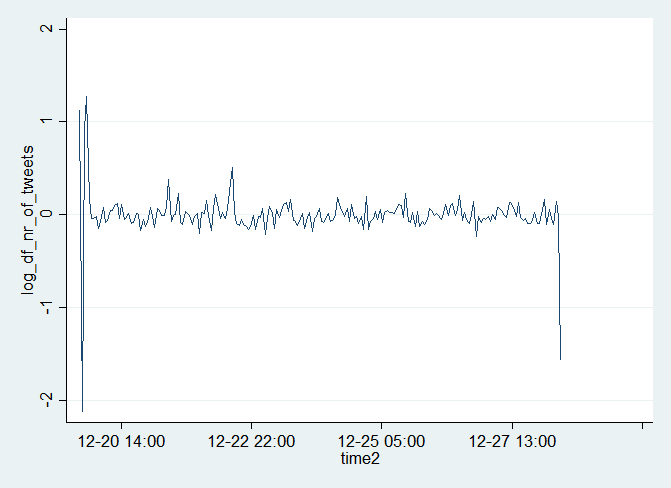
\includegraphics[width=1.12\textwidth]{stata_export_graphs/graph_plot_log_df_nr_tweets.png}
	\caption{Log first difference of number of Tweets}
	\end{subfigure}
\caption{Twitter variables development}
\end{figure}

Next we display the time series data on bitcoin price development for the observed time period. The first plot shows the hourly changes of bitcoin prices. The second and third plots are once again first difference transormations of the main variable for the later analysis. In this graph we observe a notably volatile movement and no spesific direction. This contradicts the recent trend of rising bitcoin prices in the months, but that happens because we observe a small period of a week in which bitcoin happened to have a neutral price development.\\

\begin{figure}[H]
	\begin{subfigure}{.3\textwidth}
	\centering
	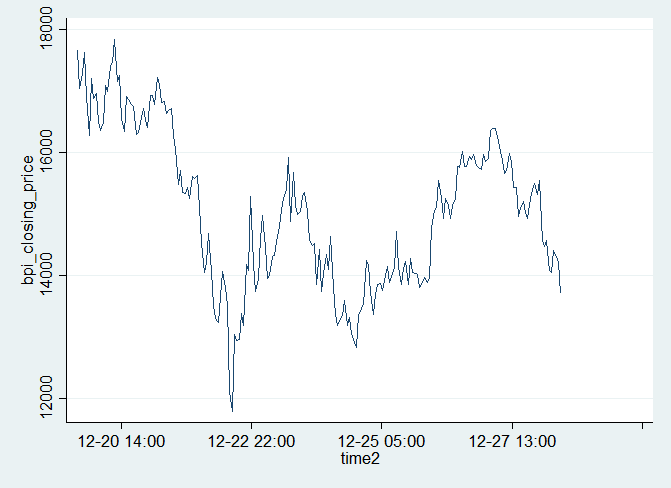
\includegraphics[width=1.12\textwidth]{stata_export_graphs/graph_plot_bpi.png}
	\caption{Hourly development of bitcoin prices}
	\end{subfigure}\hfill
	\begin{subfigure}{.3\textwidth}
	\centering
	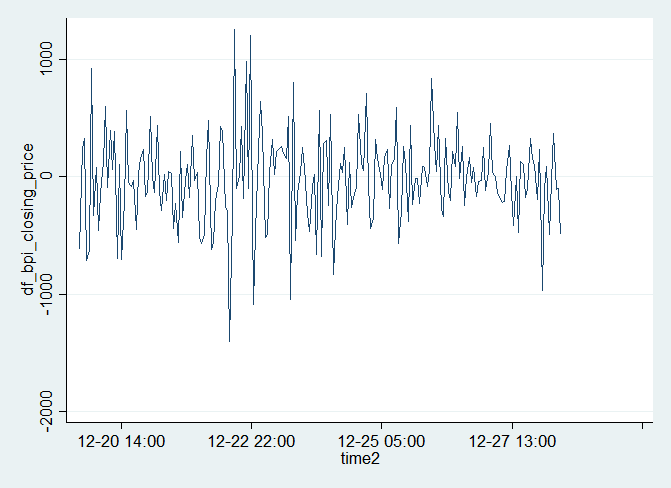
\includegraphics[width=1.12\textwidth]{stata_export_graphs/graph_plot_df_bpi.png}
	\caption{First difference of bitcoin prices}
	\end{subfigure}\hfill
	\begin{subfigure}{.3\textwidth}
	\centering
	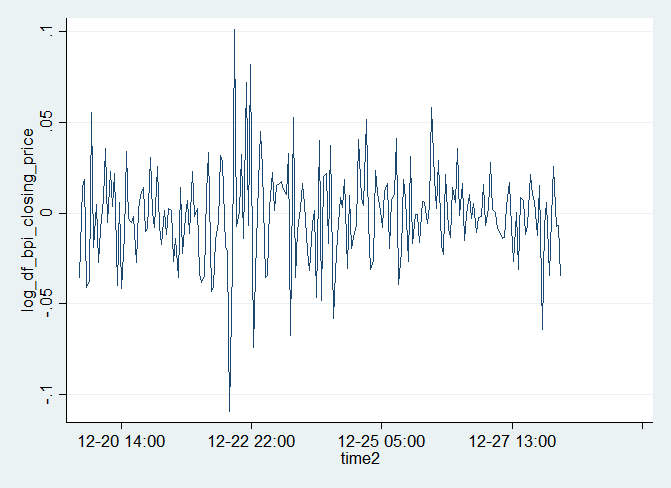
\includegraphics[width=1.12\textwidth]{stata_export_graphs/graph_plot_log_df_bpi.png}
	\caption{Log first difference of bitcoin prices}
	\end{subfigure}
\caption{Bitcoin price development}
\end{figure}
	
\clearpage

%************************** Chapters 3 - Econometric Modelling and Results **************************
\section{Econometric Modelling and Results}
\label{sec:EconometricModellingandResults}
As stated in the beginning, we want to examine the underlying relationship between twitter activity and bitcoin price fluctuations. From our data collection, we are left with two time series datasets representing two variables. A broadly used statistical method to simultaneously analyze multiple time series is the Vector Autoregression (VAR) approach. In this method the endogenous variables are determined both by their own historical values and by the historical values of the other endogenous variables (\cite[pp.~4--5]{lütkepohl2007new}).\\
To generate the econometric results that follow we used the statistical software STATA.

\subsection{Stationarity}
Before estimating a VAR model, the time series data must be checked for stationary. Accordingly, the means and variances are constant over time and the dataset does not show any trending behavior. Non-stationary data can lead to an inaccurate model which is undesirable. To test for stationarity, we use the Augmented Dickey-Fuller (ADF) test.\\

First, we check for stationarity for the twitter data (variable name: nr\_of\_tweets). Because this variable may not be stationary we also check for the first difference (df\_nr\_of\_tweets) and the logarithmic first difference of this variable (log\_df\_nr\_of\_tweets). The results of the augmented Dickey-Fuller test are listed in the  following table:\\

\begin{figure}[H]
\centering
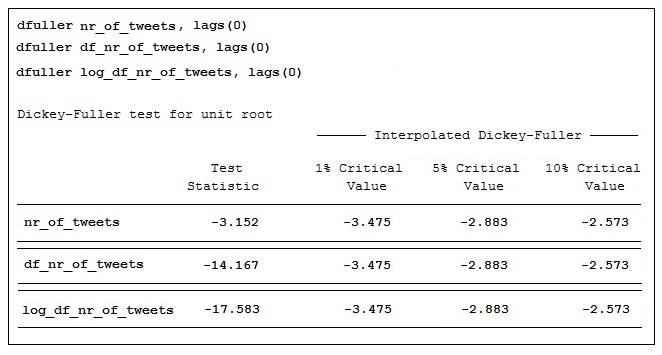
\includegraphics[scale=0.85]{stata_export_graphs/ADF_twitter_variables.png}
\caption{Twitter variables stationarity test}
\label{fig:3}
\end{figure}
	
From these result we can see that only the first variable is not stationary. This is because the absolute value of the Test Statistic (3.152) is smaller than the absolute value of the 1\% critical value (3.475). The second variable is stationary (14.167 $>$ 3.475) and from here onwards we are going to continuous the analysis by using this first difference transformetion, which fulfils stationarity.\\

Secondly, we have to check for stationarity for the second variable, the bitcoin prices (variable name: bpi\_closing\_price). Here we also included the first difference (variable name: df\_bpi\_closing\_price) and the logarithmic first difference (variable name: log\_df\_bpi\_closing\_price) transformations. The ADF test for these variables gives the following results:\\

\begin{figure}[H]
\centering
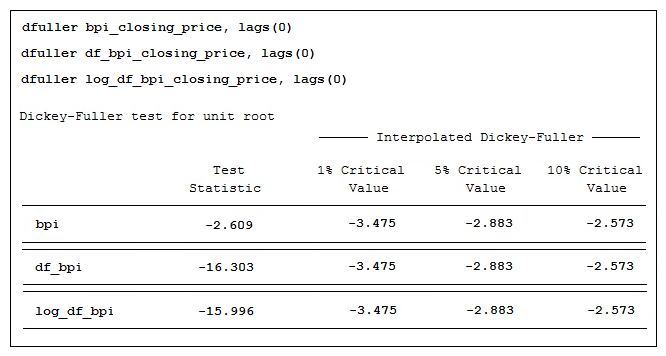
\includegraphics[scale=0.85]{stata_export_graphs/ADF_bpi_variables.png}
\caption{Bitcoin variables stationarity test}
\label{fig:4}
\end{figure}
	
These result also suggest to use the first difference transformation of the variable bitcoin prices, for stationarity to be fulfilled.

\subsection{Lag-Specification}
To select the optimal number of lags to use for the VAR regression, we have to check for various information criteria. Information criteria are measuring the tradeoff between model fit and parsimony, giving the optimal number of lags to use (\cite[p.~27]{brandtwilliams2007}). The calculations of these criteria for our specific data set are shown in the following table.\\

\begin{figure}[H]
\centering
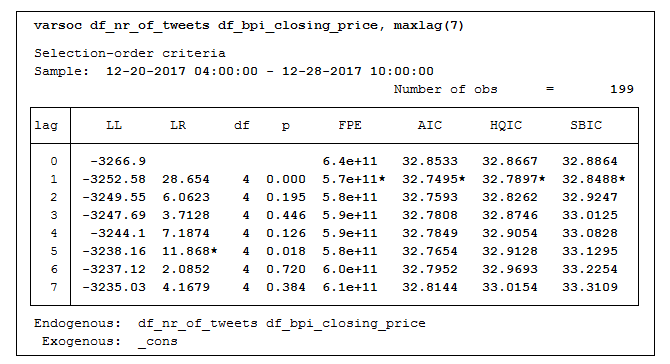
\includegraphics[scale=0.85]{stata_export_graphs/LAG_crit_df_nr_tweets_df_bpi.png}
\caption{Lag Specification}
\label{fig:5}
\end{figure}

As can be seen, STATA calculates and presents various information criteria (AIC, HQIC, SBIC). The asterisk indicates the optimal lag lenght to use for the regression analysis. In this case all criteria suggest a lag length of 1.
		
\subsection{Regression Model}
After determining the optimal lag length the next step is to build the vector autoregression model (VAR model).\\
For this analysis, we use a basic unrestricted VAR model which consists of two endogenous variables, T\textsubscript t which repesents the variable {\itshape df\_nr\_of\_tweets} in our data set and B\textsubscript t which represents {\itshape df\_bpi\_closing\_price}. As defined in the previous section the selected otpimal time lag is 1. Given these information, the model equations can be written as follows:

\begin{equation}
\begin{split}
T_t = c_1 + a_{11}T_{t-1} + a_{12}B_{t-1} + \epsilon_1 \\
B_t = c_2 + a_{21}T_{t-1} + a_{22}B_{t-1} + \epsilon_2
\end{split}
\end{equation}

This model shows that the current value of our endogenous variables is determined by its own past values, the past values of the other variable and an error term. In our research approach we ask the question, if the amount of tweets mentioning bitcoin in the past, has an effect on the bitcoin prices in the periods that follow. This question is reflected in the second equation of this model.\\

After running the above VAR regression in STATA we get following results:
	
\begin{table}
\centering
	\begin{tabular}{lcc} \hline
	 & (T\textsubscript{t}) & (B\textsubscript{t}) \\
	VARIABLES & df\_nr\_of\_tweets & df\_bpi\_closing\_price \\ \hline
	 &  &  \\
	L.df\_nr\_of\_tweets (T\textsubscript{t-1}) & 0.00999 (a\textsubscript{11}) & 0.00463 (a\textsubscript{21}) \\
	 & (0.0693) & (0.0104) \\
	L.df\_bpi\_closing\_price (B\textsubscript{t-1}) & -0.675 (a\textsubscript{12}) & -0.125* (a\textsubscript{22}) \\
	 & (0.469) & (0.0707) \\
	Constant  & -88.34 (c\textsubscript{1}) & -18.48 (c\textsubscript{2}) \\
	 & (177.9) & (26.79) \\
	 &  &  \\
	 Observations & 205 & 205 \\ \hline
	\multicolumn{3}{c}{ Standard errors in parentheses} \\
	\multicolumn{3}{c}{ *** p$<$0.01, ** p$<$0.05, * p$<$0.1} \\
	\end{tabular}
\caption{Var Regression}
\end{table}

The equations of our VAR model are displayed vertically in this table. As said before the relevant equation in the model is the second one which is listed on the right column (B\textsubscript{t}). The coefficient of 0.00463 (a\textsubscript{21}) implies that a change of tweets by 1 tweet, changes the bitcoin price by 0.005 \$. This effect is very small and statistically insignificant (p value $>$ 0.1). This answers our research question with the following statement:\\ The amount of tweets mentioning bitcoin has no significant effect on the price development of bitcoin.
		
\subsection{Granger Causality}
To assess the reliability (causality) of the previous results we use the Granger causality test. This test confirms if the statements by an estimated regression are valid. The following table shows the results of the Granger causality test for our VAR regression:\\

\begin{figure}[H]
\centering
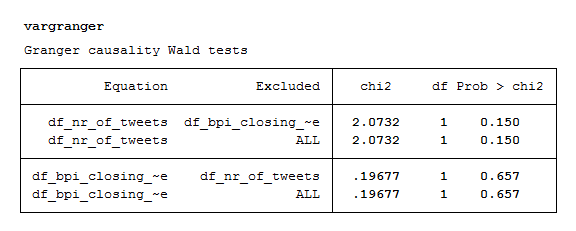
\includegraphics[scale=0.85]{stata_export_graphs/granger_test.png}
\caption{Granger causality test}
\label{fig:6}
\end{figure}

The relevant results for our regression are displayed in the lower row. The Null hypothesis here is that the lagged (lag 1) values of the number of tweets does not cause a change in the bitcoin prices. The Alternative hypothesis would then be that the lagged values of the number of tweets does cause a change in bitcoin prices. As the results show, the Probability value is 65.7\% which is clearly more than 5\% and constrain us to accept the Null hypothesis and conclude that the regression results stated above are valid.\\

\clearpage

%************************** Chapters 4 - Conclusion **************************
\section{Conclusion}
\label{sec:Conclustion}
Understanding, describing and predicting the current phenomenon of cryptocurrencies has been the objective of many researchers. A variety of methods and approaches have been applied und mixed results have been produced. Our goal for this seminar paper was to investigate the possibility of the existence of a correlation between twitter activity regarding bitcoin and the price evolution of bitcoin. After collecting hourly data for approximately 8 days we generated 2 time-series datasets and decided to perform a statistical analysis by using the Vector Autoregression (VAR) approach.\\

According to our regression results, changes in twitter activity due to more or less tweets about bitcoin have a very small and insignificant effect on future changes of bitcoin price. The validity of this statement was also verified and confirmed by the Granger causality test. At this point, however, it must be pointed out that only a small period of time has been considered in this analysis and the results cannot be generalized for the overall trend of cryptocurrencies in the recent time or for the future. We are also aware that we may have observed a period of abnormal behavior of bitcoin prices compared to the trend of the last months.\\

We encourage further research in the same direction as this paper and would be interested to see an analysis with observations over a longer period. 


\clearpage
		
\end{spacing}

\clearpage

%************************** Bibliography **************************
\section{References}
\printbibliography[heading=none]

\clearpage

%************************** Declaration of Authorship **************************
\section{Declaration of Authorship}
We hereby declare,
\begin{itemize}
\item that we have written this thesis without any help from others and without the use of documents and aids other than those stated above;
\item that we have mentioned all the sources used and that we have cited them correctly according to established academic citation rules;
\item that we have acquired any immaterial rights to materials we may have used such as images or graphs, or that we have produced such materials ourself;
\item that the topic or parts of it are not already the object of any work or examination of another course unless this has been explicitly agreed on with the faculty member in advance and is referred to in the thesis;
\item that we will not pass on copies of this work to third parties or publish them without the University’s written consent if a direct connection can be established with the University of St.Gallen or its faculty members;
\item that we are aware that our work can be electronically checked for plagiarism and that we hereby grant the University of St.Gallen copyright in accordance with the Examination Regulations in so far as this is required for administrative action;
\item that we are aware that the University will prosecute any infringement of this declaration of authorship and, in particular, the employment of a ghostwriter, and that any such infringement may result in disciplinary and criminal consequences which may result in our expulsion from the University or us being stripped of our degree.
\end{itemize}

\begin{flushleft}
................................\\
Dimitrios Koumnakes - 10-613-370\\\bigskip\bigskip 
................................\\
Severin Kranz - 13-606-355\\\bigskip\bigskip
................................\\
Joël Sonderegger - 11-495-488\\\bigskip\bigskip
................................\\
Alen Stepic - 11-475-258\\\bigskip\bigskip
................................\\
Chi Xu - XX-XXX-XXX

By submitting this academic term paper, we confirm through my conclusive action that we are submitting the Declaration of Authorship, that we have read and understood it, and that it is true.
\end{flushleft}

\clearpage

\end{document}
%************************** DOCUMENT_ENDS_HERE **************************
